\documentclass[12pt]{article}
\usepackage{scrextend}
\usepackage[utf8]{inputenc}
\usepackage[polish]{babel}
\usepackage[T1]{fontenc}%polskie znaki
\usepackage[utf8]{inputenc}%polskie znaki
\usepackage{geometry}
\usepackage{float}
\usepackage{enumitem}
\usepackage{hyperref}
\usepackage{graphicx}
\usepackage{amsmath}
\usepackage{tabularx}


\renewcommand{\baselinestretch}{1.5}


\begin{document}

\begin{flushleft}
    Damian Koper \textbf{241292} \\
\end{flushleft}
\vspace{1cm}
{
    \centering
    {\Huge\scshape\bfseries Modelowanie i analiza systemów informatycznych }\\
    \large{Logika Temporalna i Automaty Czasowe - konstrukcja prostych automatów UPPAAL.}\\
    \vspace{0.5cm}
}
\newcounter{ex}
\setcounter{ex}{1}
\newcommand{\ex}[1]{
    \refstepcounter{ex}{
        \noindent\normalfont\Large\bfseries Zadanie \arabic{ex}.
    } \\
    #1
}

\ex{Losowe przejście}
\begin{figure}[H]
    \centering
    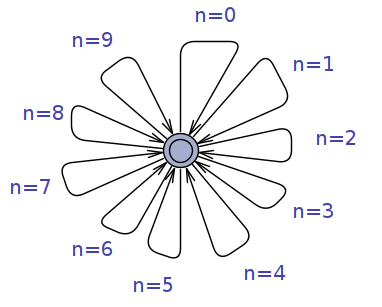
\includegraphics[width=0.3\linewidth]{../../lab11/ex_2}
\end{figure}

\ex{Losowy zakres}
\begin{figure}[H]
    \centering
    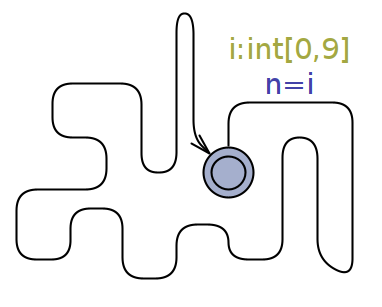
\includegraphics[width=0.3\linewidth]{../../lab11/ex_3}
\end{figure}

\clearpage
\ex{Zamek}
\begin{figure}[H]
    \centering
    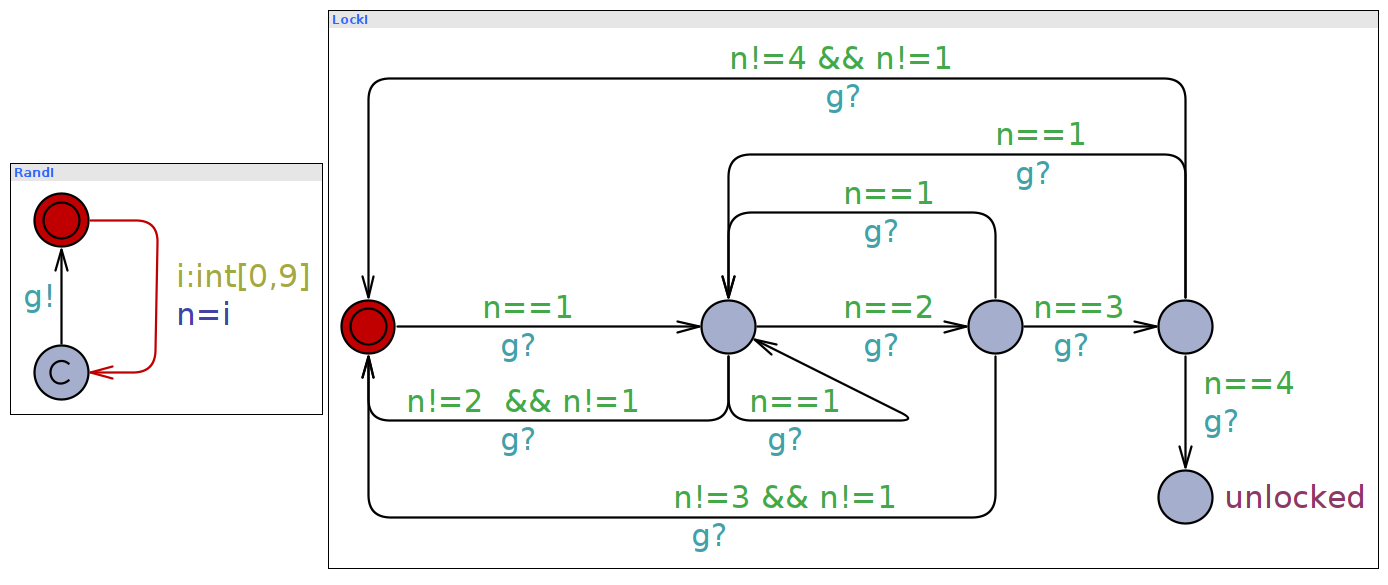
\includegraphics[width=\linewidth]{../../lab11/ex_4}
\end{figure}

\clearpage

\ex{Klient, bankomat, bank}
\begin{figure}[H]
    \centering
    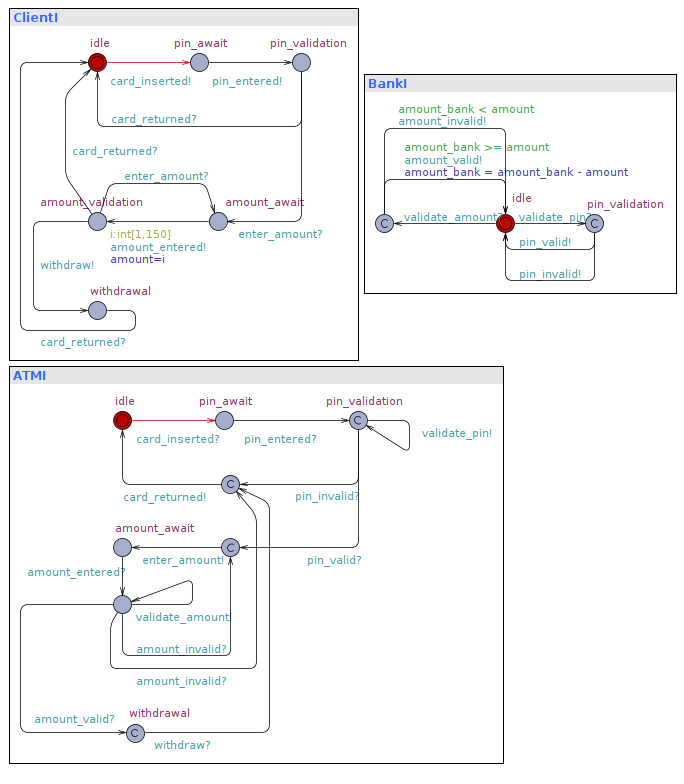
\includegraphics[width=1\linewidth]{../../lab11/ex_5}
\end{figure}

\end{document}